\documentclass{article}
\usepackage{graphicx} % Required for inserting images
\usepackage{pgfgantt}
\usepackage{hyperref}
\title{838L Proposal}
\author{Arjun Vedantham \\ Yusuf Bham}
\date{March 2024}

\begin{document}

\maketitle

\section{Introduction and Background}
We plan on constructing a domain specific language for signal processing tasks, with the capacity for speedup on domain specific hardware. Signal processing tasks have become increasingly important, especially with the advent of low-cost software defined radio (SDR) hardware, which allows engineers to avoid implementing discrete hardware components to filter, amplify, decimate, etc. signals received over radio. However, while SDRs have allowed for more flexible processing on off-the-shelf computers, it has come at the cost of shifting much of the processing load onto the CPU, which may not be capable of efficiently processing signal data. ASICs and FPGAs have been used as solutions to this problem, but ASICs suffer from being rigidly domain specific, while FPGAs are difficult to program and are largely incompatible with existing SDR frameworks. For example, GNURadio, a popular GUI based SDR framework, emits code in C++ or Python, which are not conducive to the RTL languages typically used by FPGAs. \\

Furthermore, extending the functionality of GNURadio is difficult. While the flowgraph interface given by GNURadio provides a good abstraction for implementing common signal processing functions, extending GNURadio's functionality means that engineers frequently have to contend with a cumbersome C++ backend when writing out-of-tree modules. 

\section{Our Contribution}
We plan on building a functional domain specific language for signal processing tasks. We believe that a functional paradigm would map well to signal processing tasks, which often involve mapping successive functions over streams of incoming data. Furthermore, this would allow for a more generalized composition which still respects stateful aspects prevalent in the signal processing, while still remaining terse. We plan on generating MLIR for LLVM's CIRCT framework, which would allow us to relatively easily target an FPGA. If we can, we'd also like to add a backend for LLVM's typical IR in order to increase breadth of scope - allowing the language to be used in both hardware and software applications. This may also be possible with MLIR itself, though we haven't fully looked into the details of dual purposing MLIR and the adaptations necessary. \\

There have been other projects that have built functional DSLs for signal processing. Ziria is a DSL constructed by researchers at Microsoft Research, with an emphasis on implementing the physical layer of networking devices. While this project would take inspiration from Ziria, we intend to make our language less application-specific to networking and more of a general toolkit for common signal processing tasks. Additionally, Ziria programs ``target commodity CPUs and large parts of program pipelines run on dedicated cores'', meaning that there is the potential for speedup by using heterogeneous hardware as opposed to general purpose CPUs. \\

There are also smaller projects, like the language $\mu$, which was a functional language for music synthesis. While this language did not generate assembly or allow for hardware acceleration in any way, we think that our language would involve a similar feature set as a general, largely application-neutral way to speed up signal processing tasks in hardware. 

\subsection{Approach}
The initial plan would be a Lisp-esque language for ease of parsing, though as the project progresses we would improve syntax. Specifically, our initial thoughts were on Rust's \texttt{nom} or Haskell's \texttt{megaparsec}. Our syntax would be closer to that of ML languages or Haskell than a C-style language, which differs from the standard languages used in this domain.

For a type system, a basic HM type system would suffice and allow for typical functional paradigms paradigms and particularly an abstraction over State needed in order to handle changes made after reads while still keeping ease of composition. An alternative to this would be bidirectional typing, which is used by languages such as Purescript and Dhall, although this would be somewhat more complex to implement. Both allow for higher-rank polymorphism, which is important for language expressiveness. 

Our current plan is to emit MLIR for use with LLVM's CIRCT framework, which has a variety of output options allowing easy synthesis and testing. We've also considered the option of outputting XML matching that of GNURadio's, which would make targeting hardware more difficult - but would allow for easier integration with existing work.

\begin{figure}
\begin{center}

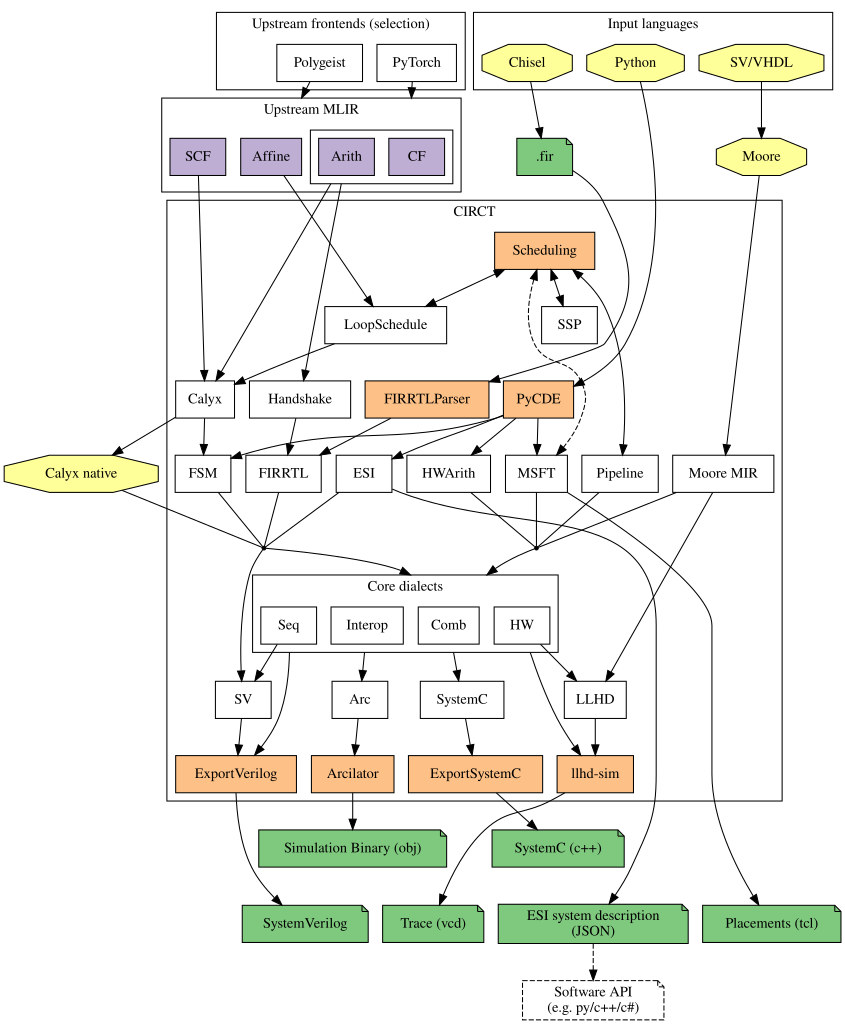
\includegraphics[width=0.5\textwidth]{circt.png}
\end{center}

\caption{The CIRCT framework}
\end{figure}

\subsection{Evaluation and timeline} % Needs more detail
We plan on doing small tests at first with a signal data captured using an off-the-shelf RTL-SDR module, simulating the model generated by the compiler for our functional language on a normal CPU and performing simple tasks on the signal (low/high/band pass filtering, decimation). For circuit simulation, we plan to use a platform like Verilator, a platform which takes hardware descriptions in Verilog (which would be generated by our compiler using CIRCT) and generates equivalent C++ code that can be run on general purpose CPUs. If this is successful, we would like to implement more complex processing tasks, including a Fourier transform, which we would see as a critical benchmark for demonstrating the expressiveness of our language. 
We would then move the targeted platform to real hardware, such as an ICESTICK FPGA from Lattice. Performance would be compared to equivalent flowgraphs in GNURadio, and equivalent hand-tuned code in Python/C++. This would demonstrate both the capabilities of the language as well as the overhead presented by it. We may also measure code \textit{size} in order to evaluate the expressiveness of the language, though this is a rather arbitrary metric, it would allow for emphasis of the ease presented by a more functional approach. 
Finally, although not a critical part of our evaluation, we hope to make the language expressive enough to add support for arbitrary demodulation schemes. For example, even though languages like Ziria are targeted to implement the physical layer of wireless protocols, we hope that some of the demodulation schemes used in the language (e.g. adding support for demodulating signals encoded using frequency key shifting). 

\subsection{Timeline}

\begin{figure}[htb!]
    \begin{center}
    
    \begin{ganttchart}[y unit title=0.4cm,
    y unit chart=0.5cm,
    vgrid,hgrid, 
    title label anchor/.style={below=-1.6ex},
    title left shift=.05,
    title right shift=-.05,
    title height=1,
    progress label text={},
    bar height=0.7,
    group right shift=0,
    group top shift=.6,
    expand chart=1.2\textwidth,
    group height=.3]{1}{24}
    %labels
    \gantttitle{Remainder of the semester}{24} \\
    \gantttitle{Week 7-8}{6} 
    \gantttitle{Week 9-10}{6} 
    \gantttitle{Week 11-12}{6} 
    \gantttitle{Week 13-14}{6} \\
    %tasks
    \ganttbar{Set up simulator}{1}{6} \\
    \ganttbar{Define grammar}{1}{6} \\
    \ganttbar[progress=33]{Lit review of DSP tasks}{1}{6} \\
    \ganttbar{Integrate CIRCT as backend}{6}{18} \\
    \ganttbar{Simulated workload tests}{12}{18} \\
    \ganttbar{FPGA deployment}{15}{24} \\
    \ganttbar{Efficiency testing}{12}{24}
    
    %relations 
    \ganttlink{elem0}{elem3} 
    \ganttlink{elem1}{elem3} 
    \ganttlink{elem2}{elem1} 
    \ganttlink{elem3}{elem4} 
    \ganttlink{elem4}{elem5} 
    \ganttlink{elem4}{elem6}
    \end{ganttchart}
    \end{center}
    \caption{Gantt Chart}

\end{figure}
\subsection{Bibliography}
\begin{itemize}
    \item \href{https://www.microsoft.com/en-us/research/wp-content/uploads/2016/02/ASPLOS-camera.pdf}{Ziria} - a DSL specifically for implementing physical layer networking protocols (2015)
    \item \href{https://link.springer.com/chapter/10.1007/978-3-319-51676-9_12}{A Domain-Specific Language for Software-Defined Radio} - builds off of the work of the original Ziria paper by defining semantics in greater detail (2016)
    \item \href{https://www.cs.unb.ca/tech-reports/honours-theses/Matthew.Gordon-4997.pdf}{$\mu$: A Functional Programming Language for Digital Signal Processing}
     Compiles to C++, CPU-bound - also primarily intended for audio synthesis/engineering (2003)
     \item \href{https://circt.llvm.org/}{CIRCT Project - LLVM}
\end{itemize}
\end{document}
